%======================================================================
% CAPITULO 2: INTERFAZ DE USUARIO Y SANDRA AI
%======================================================================

\chapter{Interfaz de Usuario y Sandra AI}
\label{ch:dashboard}

Este capitulo describe la interfaz principal de \sdc{}, conocida como el Dashboard, y presenta \sandraai{}, el asistente de inteligencia artificial integrado.

\section{El Dashboard Principal}
\label{sec:dashboard}

El panel central de SDC proporciona una vision integral del estado del sistema mediante metricas en tiempo real.

\begin{figure}[H]
\centering
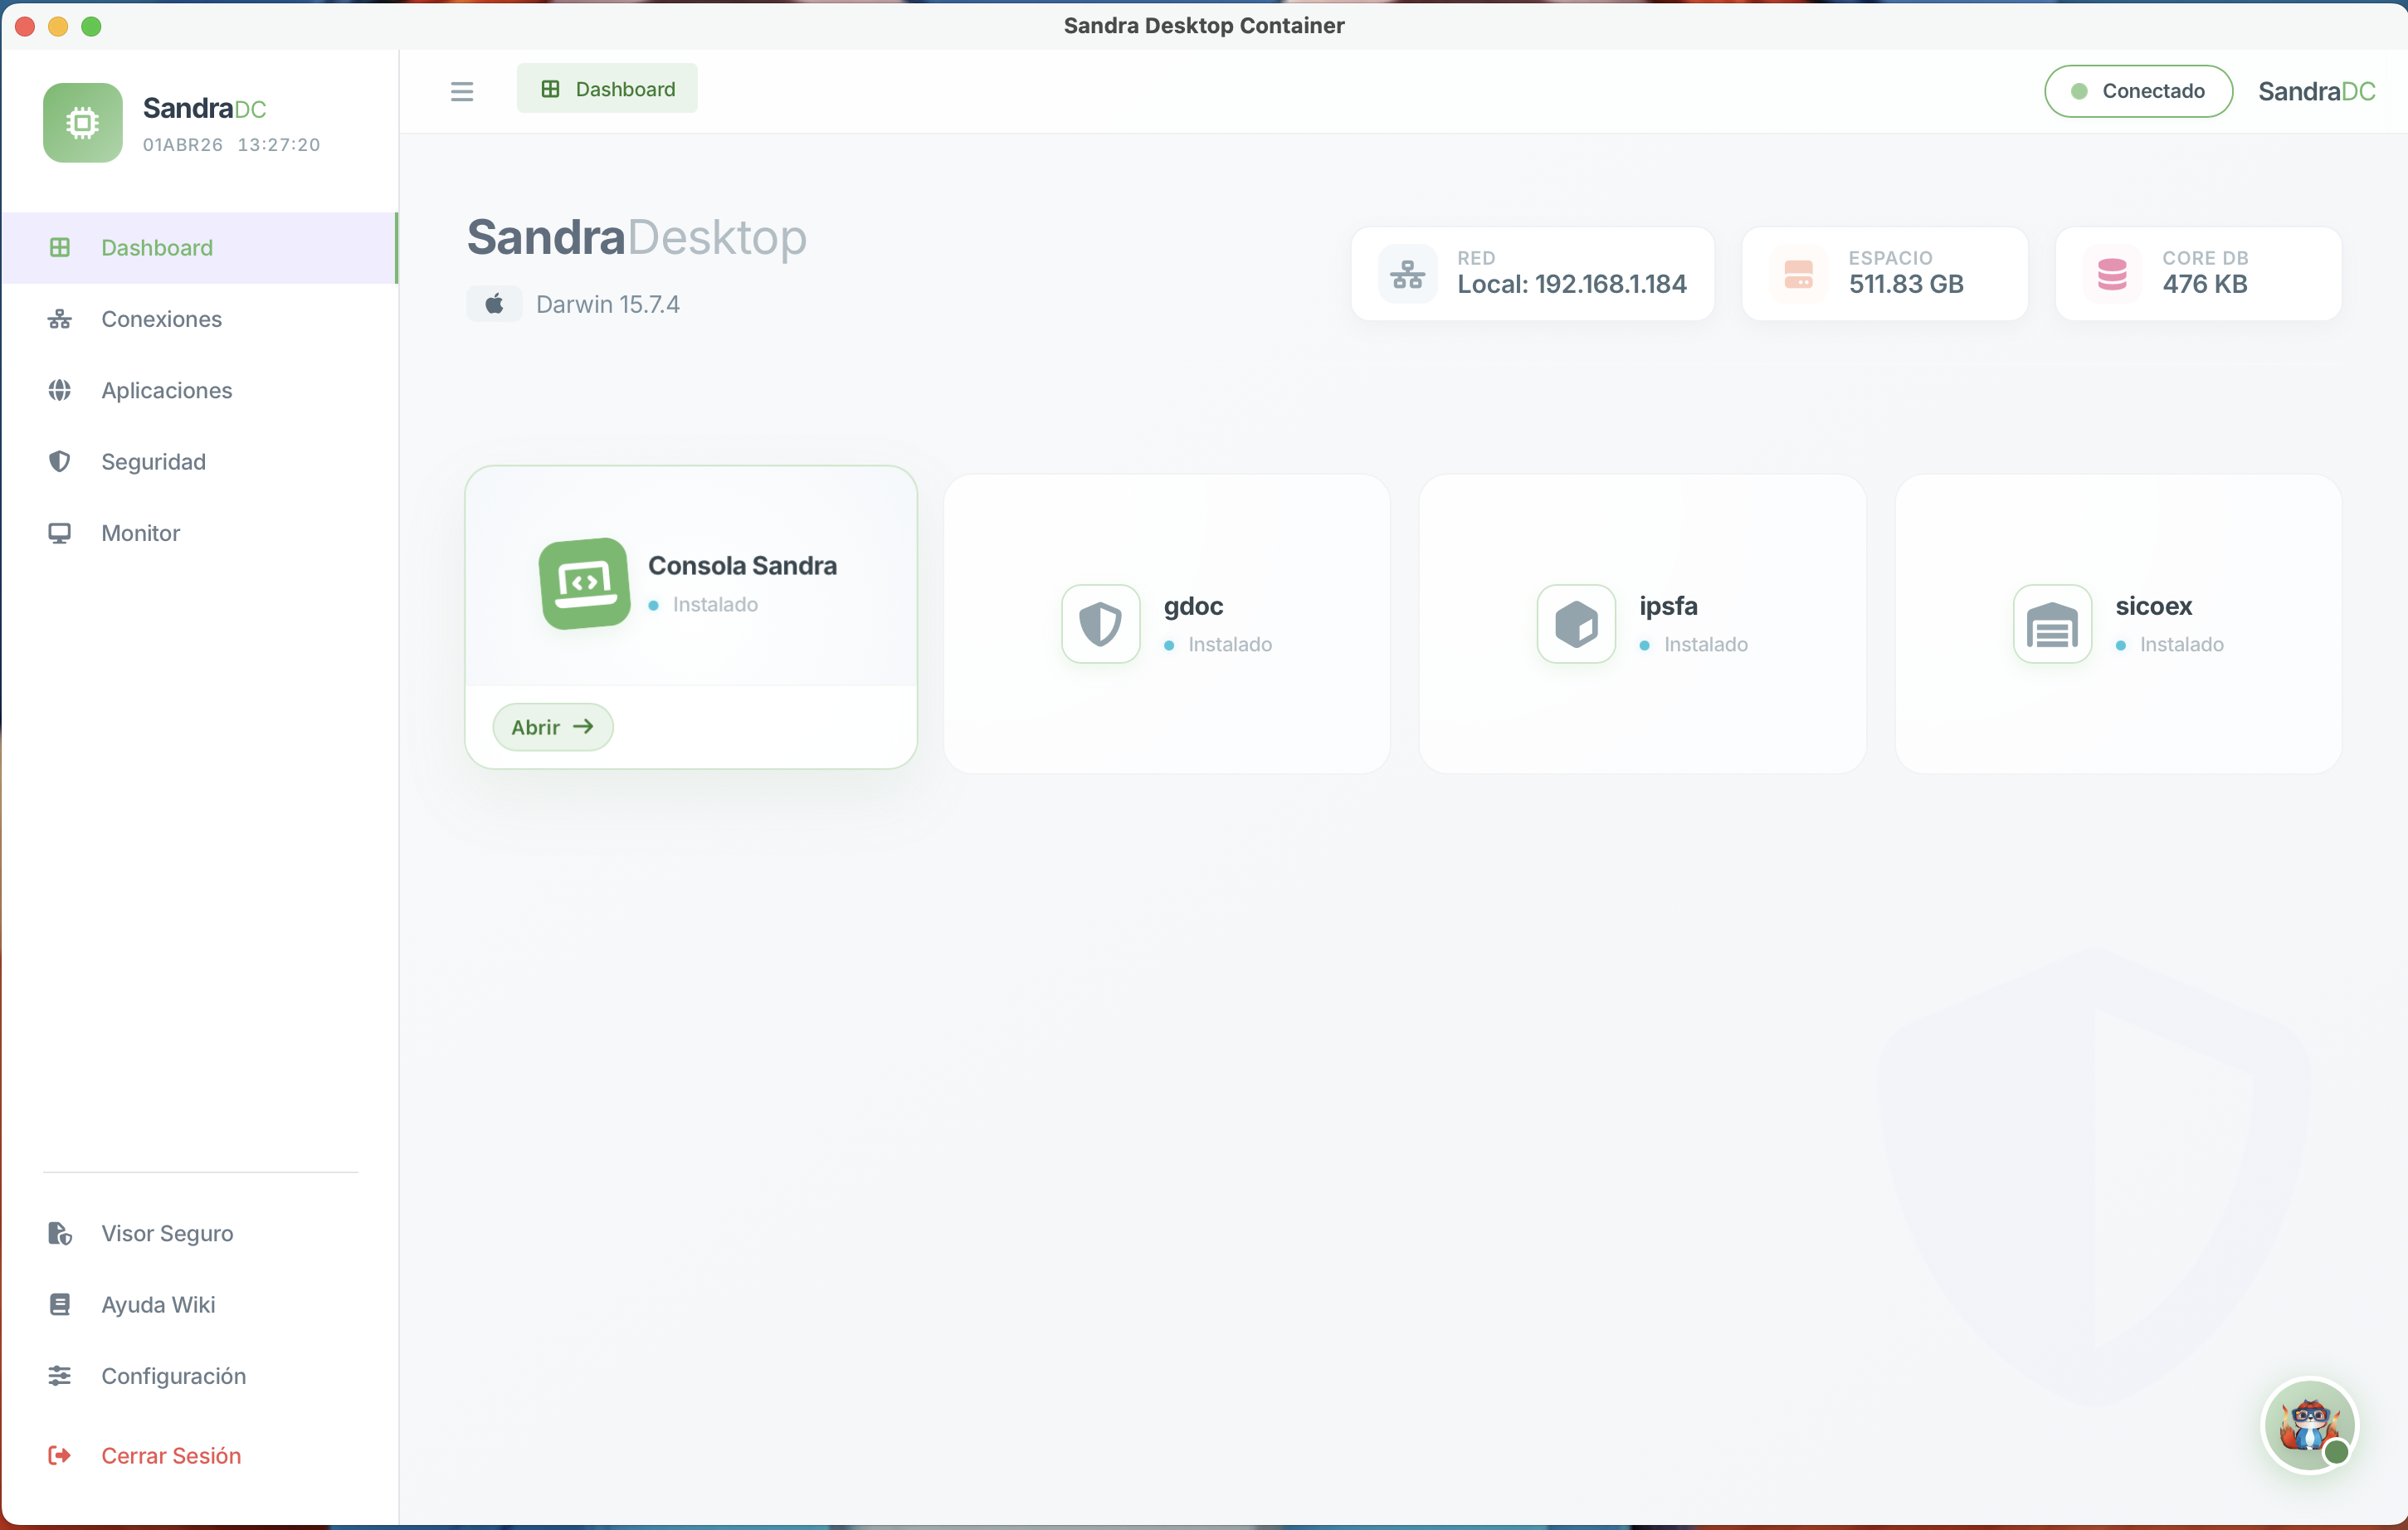
\includegraphics[width=0.95\textwidth]{anexos/4 principal.png}
\caption{Dashboard principal de Sandra Desktop Container}
\label{fig:dashboard}
\end{figure}

\subsection{Panel de Metricas del Sistema}

El dashboard presenta tres metricas fundamentales organizadas en tarjetas visuales:

\begin{table}[H]
\centering
\begin{tabular}{>{\centering\arraybackslash}m{1.5cm}p{2.5cm}p{9cm}}
\toprule
\textbf{Icono} & \textbf{Metrica} & \textbf{Descripcion} \\
\midrule
{\color{sandraGreen}\Large\faIcon{network-wired}} & RED & Estado de la conexion local, latencia y throughput \\
\midrule
{\color{sandraGreen}\Large\faIcon{hdd}} & ESPACIO & Capacidad disponible en disco para contenedores \\
\midrule
{\color{sandraGreen}\Large\faIcon{database}} & CORE DB & Base de datos SQLite interna cifrada \\
\bottomrule
\end{tabular}
\caption{Metricas principales del Dashboard}
\label{tab:metricas-dashboard}
\end{table}

\subsection{Interpretacion de las Metricas}

\subsubsection{Estado de RED}

La metrica de red muestra:
\begin{itemize}[leftmargin=*]
    \item Estado de conexion: Activa/Inactiva
    \item Interfaces detectadas: Ethernet, WiFi
    \item Latencia: Tiempo de respuesta en ms
    \item Throughput: Velocidad de transferencia
\end{itemize}

\begin{quote}
\textbf{Indicadores de Estado:}
\begin{itemize}
    \item \textbf{Verde}: Conexion estable y optima
    \item \textbf{Ambar}: Conexion lenta o inestable
    \item \textbf{Rojo}: Sin conexion o error
\end{itemize}
\end{quote}

\subsubsection{Espacio de Almacenamiento}

El espacio disponible se calcula considerando:
\begin{itemize}[leftmargin=*]
    \item Contenedores activos
    \item Datos temporales
    \item Logs de auditoria
    \item Cache de aplicaciones
\end{itemize}

\begin{quote}
\textbf{Advertencia:} Cuando el espacio desciende por debajo del 20 por ciento, SDC mostrara alerta.
\end{quote}

\section{Asistente Sandra AI}
\label{sec:sandra-ai}

\sandraai{} es una consola de inteligencia artificial ubicada en la esquina inferior derecha del dashboard.

\subsection{Activacion del Asistente}

Para iniciar una conversacion:
\begin{enumerate}[leftmargin=*]
    \item Hacer clic en el icono {\color{sandraGreen}\faIcon{robot}} en la esquina inferior derecha
    \item Escribir la consulta en el campo de texto
    \item Presionar Enter
\end{enumerate}

\subsection{Tipos de Interaccion}

Sandra AI procesa tres categorias de consultas:

\begin{table}[H]
\centering
\begin{tabular}{p{4cm}p{4cm}p{6cm}}
\toprule
\textbf{Categoria} & \textbf{Ejemplo} & \textbf{Respuesta} \\
\midrule
Consultas Tecnicas & Que es una ruta proxy? & Explicacion conceptual \\
\midrule
Comandos Operativos & Crear nueva conexion & Asistente de configuracion \\
\midrule
Diagnostico & Por que no puedo conectarme? & Analisis de logs \\
\bottomrule
\end{tabular}
\caption{Tipos de interaccion con Sandra AI}
\label{tab:tipos-ai}
\end{table}

\subsection{Comandos Predefinidos}

Sandra AI reconoce los siguientes comandos:

\begin{table}[H]
\centering
\begin{tabular}{p{5cm}p{9cm}}
\toprule
\textbf{Comando} & \textbf{Accion} \\
\midrule
nueva conexion & Inicia asistente para crear conexion \\
\midrule
listar conexiones & Muestra todas las conexiones configuradas \\
\midrule
eliminar conexion [nombre] & Elimina la conexion especificada \\
\midrule
nueva aplicacion & Inicia formulario de nueva app \\
\midrule
abrir aplicacion [nombre] & Abre la aplicacion indicada \\
\midrule
estado del sistema & Muestra metricas generales \\
\midrule
espacio disponible & Reporta espacio libre en disco \\
\midrule
logs de auditoria & Abre el visor de logs \\
\bottomrule
\end{tabular}
\caption{Comandos de voz/texto de Sandra AI}
\label{tab:comandos-ai}
\end{table}

\section{Navegacion Principal}
\label{sec:navegacion}

Modulos de la barra lateral:

\begin{table}[H]
\centering
\begin{tabular}{>{\centering\arraybackslash}m{1.5cm}p{3cm}p{8.5cm}}
\toprule
\textbf{Icono} & \textbf{Modulo} & \textbf{Descripcion} \\
\midrule
{\color{sandraGreen}\Large\faIcon{th-large}} & Dashboard & Panel principal con metricas \\
\midrule
{\color{sandraGreen}\Large\faIcon{code}} & Aplicaciones & Micro-aplicaciones desplegadas \\
\midrule
{\color{sandraGreen}\Large\faIcon{plug}} & Conexiones & Servidores remotos \\
\midrule
{\color{sandraGreen}\Large\faIcon{shield-alt}} & Seguridad & Politicas y auditoria \\
\midrule
{\color{sandraGreen}\Large\faIcon{eye}} & Visor & Documentos seguros \\
\midrule
{\color{sandraGreen}\Large\faIcon{cog}} & Configuracion & Preferencias \\
\bottomrule
\end{tabular}
\caption{Modulos de navegacion de SDC}
\label{tab:modulos-navegacion}
\end{table}

\subsection{Accesos Directos}

Botones de acceso rapido disponibles:

\begin{itemize}[leftmargin=*]
    \item {\color{sandraGreen}\faIcon{plus}} Nueva Conexion
    \item {\color{sandraGreen}\faIcon{plus}} Nueva Aplicacion
    \item {\color{sandraGreen}\faIcon{sync}} Sincronizar
    \item {\color{sandraGreen}\faIcon{history}} Auditoria
\end{itemize}

\section{Personalizacion del Dashboard}

\subsection{Temas de Color}

\begin{itemize}[leftmargin=*]
    \item \textbf{Tema Claro}: Paleta Sandra Teal Soft (default)
    \item \textbf{Tema Oscuro}: Optimizado para uso nocturno
    \item \textbf{Tema Alto Contraste}: Accesibilidad
\end{itemize}

\section{Arquitectura del Sistema}
\label{sec:arquitectura-sdc}

SDC esta construido sobre una arquitectura multicapa que combina el rendimiento de Rust con la versatilidad de Angular, proporcionando una experiencia robusta y segura.

\notacientifica{La arquitectura de SDC sigue el principio de separacion de responsabilidades, manteniendo el nucleo de seguridad (Rust) completamente aislado de la capa de presentacion (Angular).}

\subsection{Arquitectura Multicapa}

\begin{figure}[H]
\centering
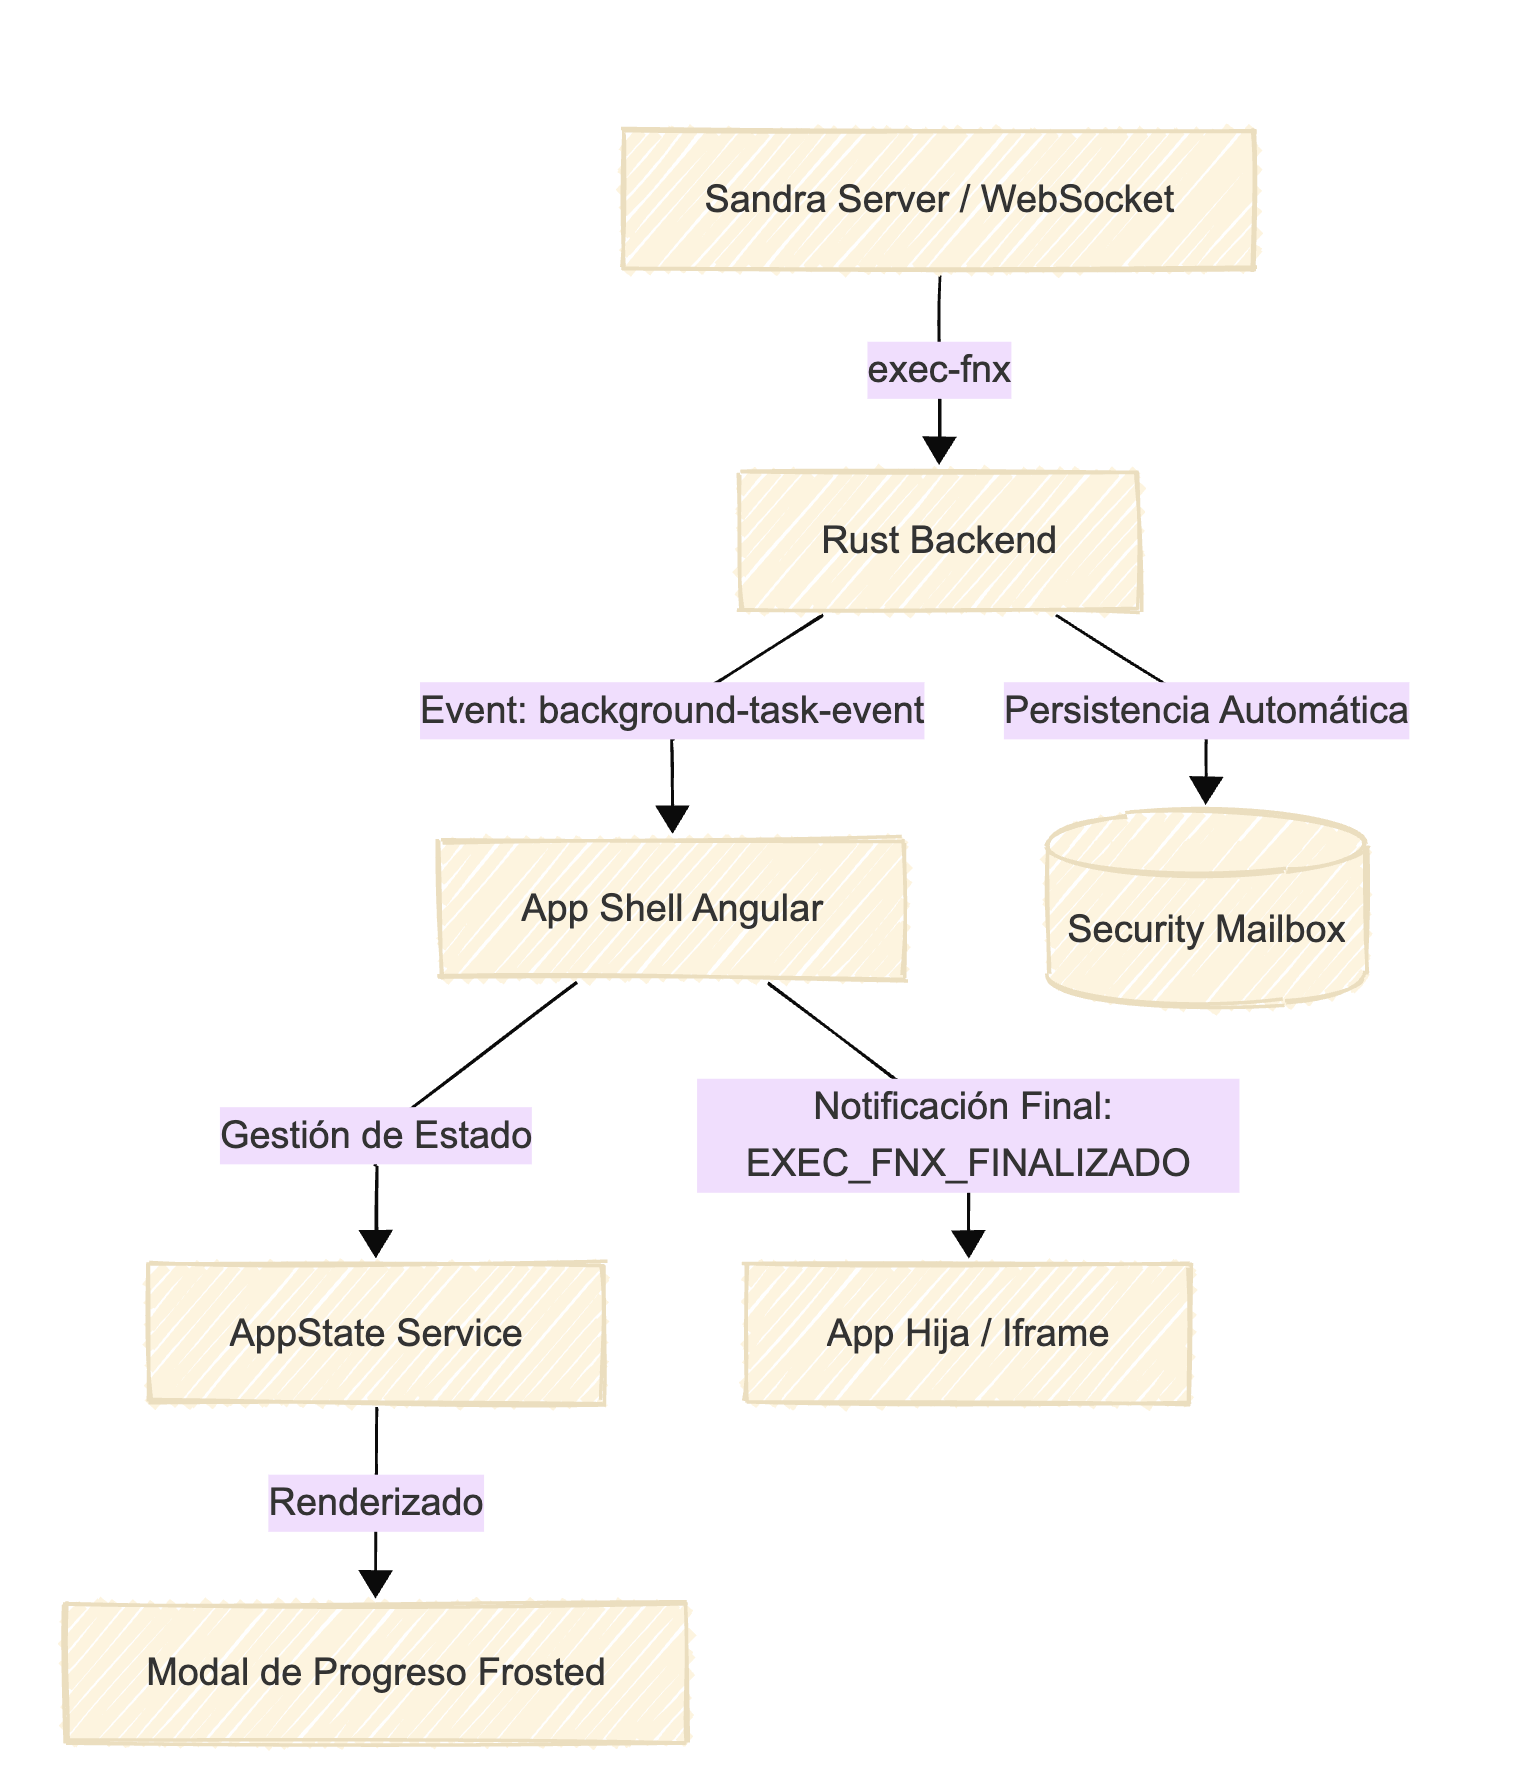
\includegraphics[width=0.95\textwidth]{anexos/arquitectura.y.comunicacion.png}
\caption{Arquitectura general del sistema SDC}
\label{fig:arquitectura}
\end{figure}

La arquitectura de SDC se organiza en cuatro capas distintas:

\begin{caja}{Capas del Sistema}
\begin{enumerate}
\item \textbf{Capa de Presentacion (Angular UI)}: Interfaz de usuario desarrollada en Angular con Componentes Standalone, Signals y Observables para reactividad instantanea.

\item \textbf{Capa de Puente (Tauri IPC)}: Puente de comunicacion entre la UI y el sistema operativo. Implementa un esquema de protocolo personalizado (sandra-app://) para el aislamiento de micro-frontends.

\item \textbf{Capa de Core (Rust + Tokio)}: Nucleo del sistema escrito en Rust, gestionando criptografia, base de datos SQLite, WebSockets y entorno de sandboxing.

\item \textbf{Capa de Sistema (OS Nativo)}: Integracion con el sistema operativo subyacente para gestion de archivos, red y procesos.
\end{enumerate}
\end{caja}

\notacientifica{Esta separacion garantiza que las vulnerabilidades en la interfaz de usuario no puedan comprometer el nucleo de seguridad del sistema.}

\subsection{Componentes de la Capa de Presentacion}

La interfaz de usuario en Angular implementa una arquitectura basada en componentes:

\begin{caja}{Servicios Principales de Angular}
\begin{itemize}
\item \textbf{SdcService}: Gestion de conexiones y estado del sistema
\item \textbf{AppStateService}: Sincronizacion de telemetria en tiempo real
\item \textbf{SecureStorageService}: Acceso cifrado al almacen local
\item \textbf{WebSocketService}: Gestion de conexiones en tiempo real
\end{itemize}
\end{caja}

\notacientifica{Los servicios utilizan patrones reactivos (Observables) para mantener la UI sincronizada con el estado del sistema en todo momento.}

\subsection{Componentes de la Capa de Core (Rust)}

El backend en Rust proporciona las siguientes capacidades fundamentales:

\begin{caja}{Modulos de Rust Core}
\begin{itemize}
\item \textbf{Crypto Module}: Implementacion de AES-256-GCM, Argon2id
\item \textbf{Database Module}: SQLite con cifrado para persistencia local
\item \textbf{WebSocket Module}: Gestion de conexiones concurrentes con Tokio
\item \textbf{Sandbox Module}: Aislamiento de aplicaciones de terceros
\item \textbf{Inspector Module}: Interceptacion y registro de trafico de red
\end{itemize}
\end{caja}

\notacientifica{El runtime asincrono Tokio permite manejar miles de conexiones WebSocket concurrentes con latencia cercana a cero, garantizando una experiencia fluida.}

\subsection{Comunicacion entre Capas}

La comunicacion entre Angular y Rust se realiza mediante el puente IPC de Tauri:

\begin{caja}{Tipos de Comunicacion}
\begin{itemize}
\item \textbf{Commands}: Llamadas sincronas desde Angular a Rust para operaciones atomicas
\item \textbf{Events}: Eventos asincronos desde Rust hacia Angular para notificaciones
\item \textbf{Streams}: Flujos de datos continuos para sincronizacion masiva
\end{itemize}
\end{caja}

\notacientifica{El puente IPC esta diseñado para impedir la inyeccion de codigo arbitrario, proporcionando un canal seguro entre la UI y el sistema.}

\subsection{Protocolo Sandra-App}

SDC implementa un esquema de protocolo personalizado para el aislamiento de micro-frontends:

\begin{caja}{Formato del Protocolo}
\begin{verbatim}
sandra-app://[modulo]/[accion]?[parametros]
\end{verbatim}
\end{caja}

\notacientifica{Este protocolo permite que las aplicaciones de terceros se ejecuten en contextos aislados, evitando el acceso no autorizado a recursos del sistema.}
